% \section{Uncomputing and Recomputing}
% \subsection{Tock}
% The key insight of Zombie is to introduce an abstraction layer between the executing program and the heap. This abstraction layer will allow the heap to transparently discard and recompute the program's intermediate values. To do so, we use the CEK machine to refer to each intermediate value by the index of the computation step that created it. Since each CEK step allocates at most one cell, this correspondence is injective. In other words, instead of storing pointers that refer to memory locations, we will store pointers, which we call ``tocks'', that refer to points in time---that is, CEK step indices.

% In our runtime, these ``tocks'' are implemented as 64-bit integers, though in our model we will treat them as logically unbounded integers. There is a global ``current tock'' counter, which starts at 0 and is increased by 1 at every transition step in the abstract machine and at every allocation. The cell allocated at step $i$ is then referred to by the tock $i$, and that tock can then be used as a pointer, stored in data structures, looked up by later computations steps, and the like.

% Note that, due to the determinism and linearity of the CEK machine, tocks are strictly ordered and the value computed at some tock $i$ can only depend on values computed at earlier tocks. Moreover we can recreate the value at tock $i$ by merely rerunning the CEK machine from some earlier state to that point. Because the CEK machine is deterministic, this re-execution will produce the same exact value as the original. Because our pointers refer to abstract values, not to specific memory locations, the heap can thus re-compute a value as necessary instead of storing it in memory.

% In other words, the way Zombie works is that the heap will store only some of the intermediate values. The ones that aren't stored will instead be recomputed as needed, and the heap will store earlier CEK states in order to facilitate that. As the program runs, intermediate values can be discarded from the heap to reduce its memory usage.

% Because a value can be recomputed from \emph{any} earlier CEK state, it will also turn out to be possible to store relatively few states. Therefore, overall memory usage---for the stored intermediate values and the stored states---can be kept low. In Zombie, we can store asymptotically fewer states than intermediate values, allowing us to asymptotically reduce memory usage.

% \subsection{Tock Tree}
% In Zombie, the heap is implemented by a runtime data structure called the tock tree. The tock tree maps tocks to the cells allocated by that step; in other words, the tock tree implements the mapping between tocks and their actual memory locations. Because values can be evicted to save memory, however, not all tocks have a mapping in the tock tree. Instead, every tock that \emph{is} present in the tock tree will also store its state. To recompute an evicted value at some tock $i$, the tock tree will find the largest state at tock $j < i$ and replay from that tock to tock $i$.

% Each node in the Tock Tree stores both a memory cell and a state. Specifically, consider the execution of the CEK machine from step $t$. In step $t + 1$ it allocates a cell; it then performs a computation in step $t + 2$. So the node at tock $t$ contains both the cell allocated at step $t + 1$ as well as the state \emph{afterwards}, at step $t + 2$. A transition might not allocate any new cells, in such a case the Node only store a state and no memory cell. To be more specific, if the node represent the execution of the CEK machine at step $t$, it will only contain the CEK state at step $t + 1$. Also note that a state, in this context, does not include every info needed for execution: in particular it does not include the tock tree, alongside any data that guide recomputation. More specifically a state denote either a $\Eval~C~\Env~K~Tock$ or a $\Apply~K~V~Tock$.

% One thing worth noticing is that continuations are also reified. This mean we treat them as like values, lifting pointers into tock, and storing continuations onto the tock tree. This allow us to also uncompute continuation as well, by evicting the node on the tock tree holding said continuation. This is crucial as traversing a deep data structure non tail-recursively produce a continuation chain of equal depth. In contrast to a ordinary runtime, in which this is a slight but inevitable unfortunate, in our case, the continuation storage can become the bottleneck of the system.

% In order to make this operation efficient, the tock tree is organized as a binary search tree. In a binary search tree, arbitrary keys (tocks) can be looked up in $O(\log(n))$ time, where $n$ is the size of the tock tree, and when a key is not found, the largest key smaller than it can be easily found. Then the heap can replay execution from that point to compute the desired tock.

% \begin{figure}
% 	\begin{tabular}{p{5em} p{3em} p{10em} p{0.45\textwidth}}
% 		Value & = & \st{P<VCell>} & Tock \\
% 		Continuation & = & \st{P<KCell>} & Tock \\
% 		State & ::= & \st{$\Eval~C~\Env~K \mid \Apply~K~V $} & $\Eval~C~\Env~K~Tock \mid \Apply~K~V~Tock $ \\
% 		Node & = & & (Maybe(KCell | VCell), State) \\
% 		Query & $:$ & (TockTree, Tock) & -> (Tock, Node) \\
% 		Insert & $:$ & (TockTree, Tock, Node) & -> TockTree \\
% 	\end{tabular}
% 	\caption{Tock Tree API. Note that we deliberately avoid dictating what node get uncomputed, in order to decouple uncomputation/recomputation with selecting what to uncompute. Instead, node might be dropped during insertion into TockTree. One might e.g. set a limit onto the amount of nodes in the Tock Tree. }
% \end{figure}
% \begin{figure}
% 	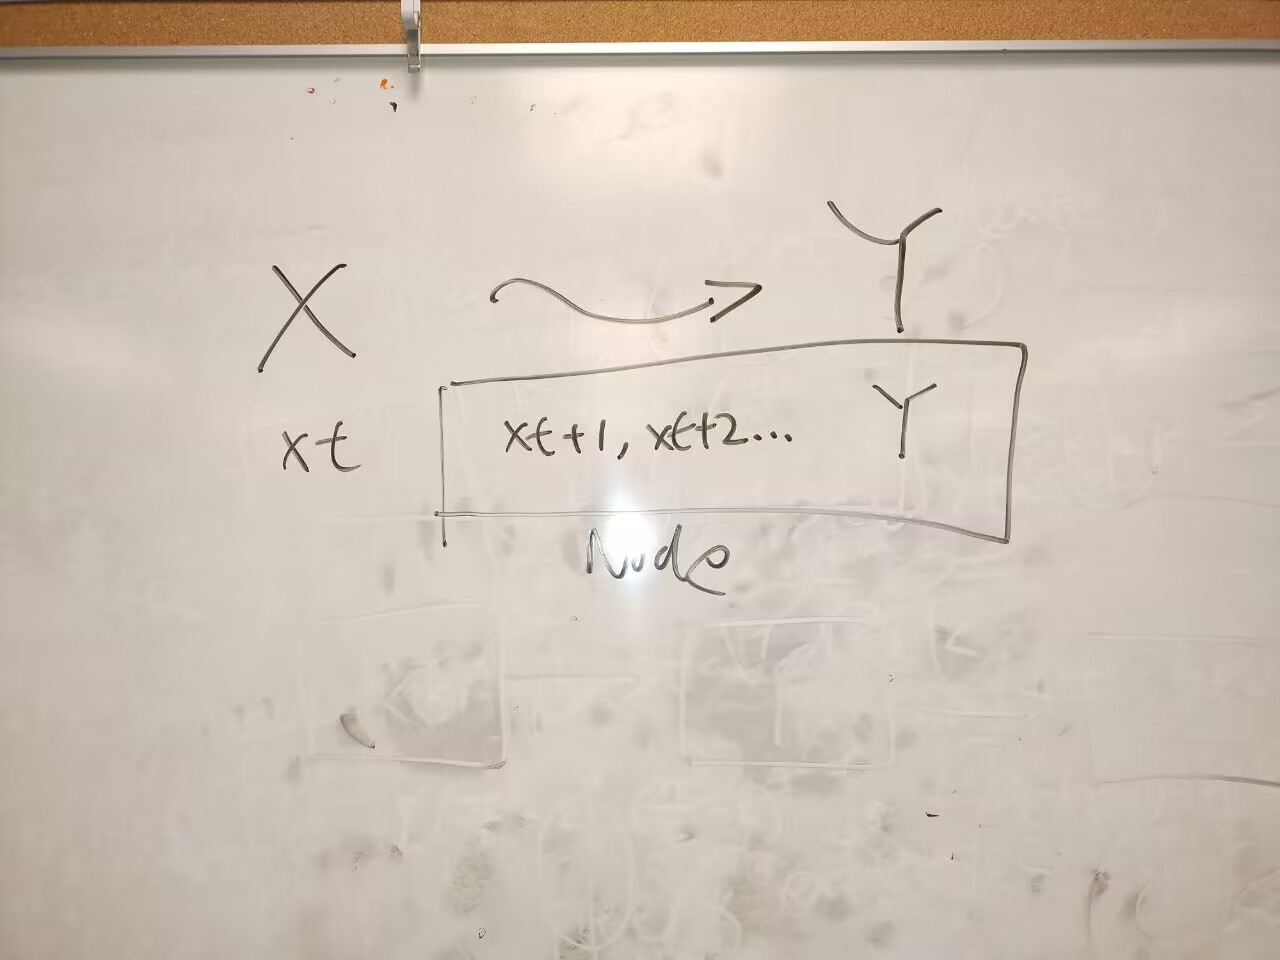
\includegraphics[width=0.5\columnwidth]{img2}
% 	\caption{a node in the tock tree}
% \end{figure}
% \begin{figure}
% 	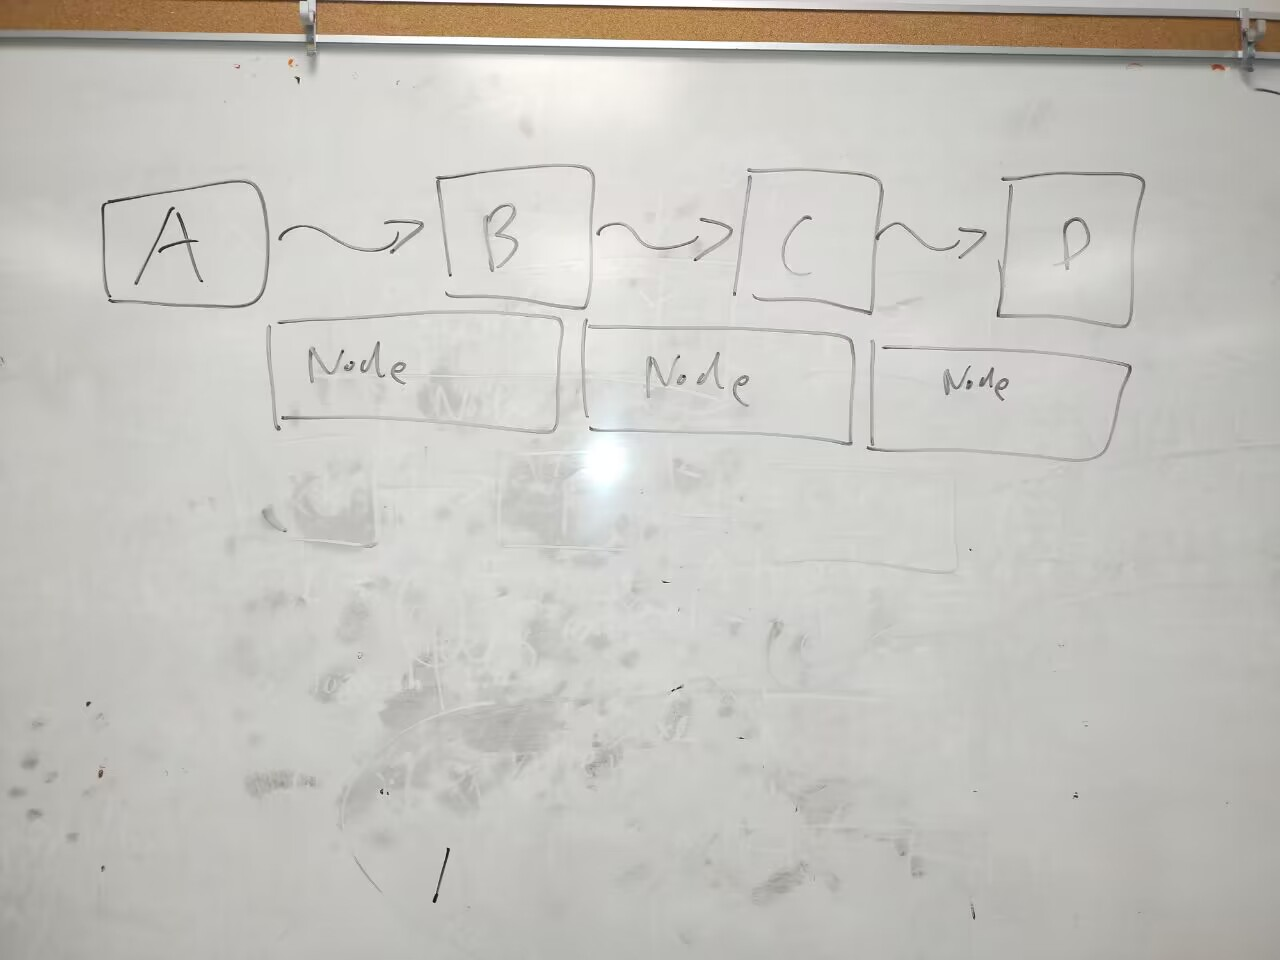
\includegraphics[width=0.5\columnwidth]{img3}
% 	\caption{the tock tree with multiple nodes}
% \end{figure}

% \begin{figure}
% 	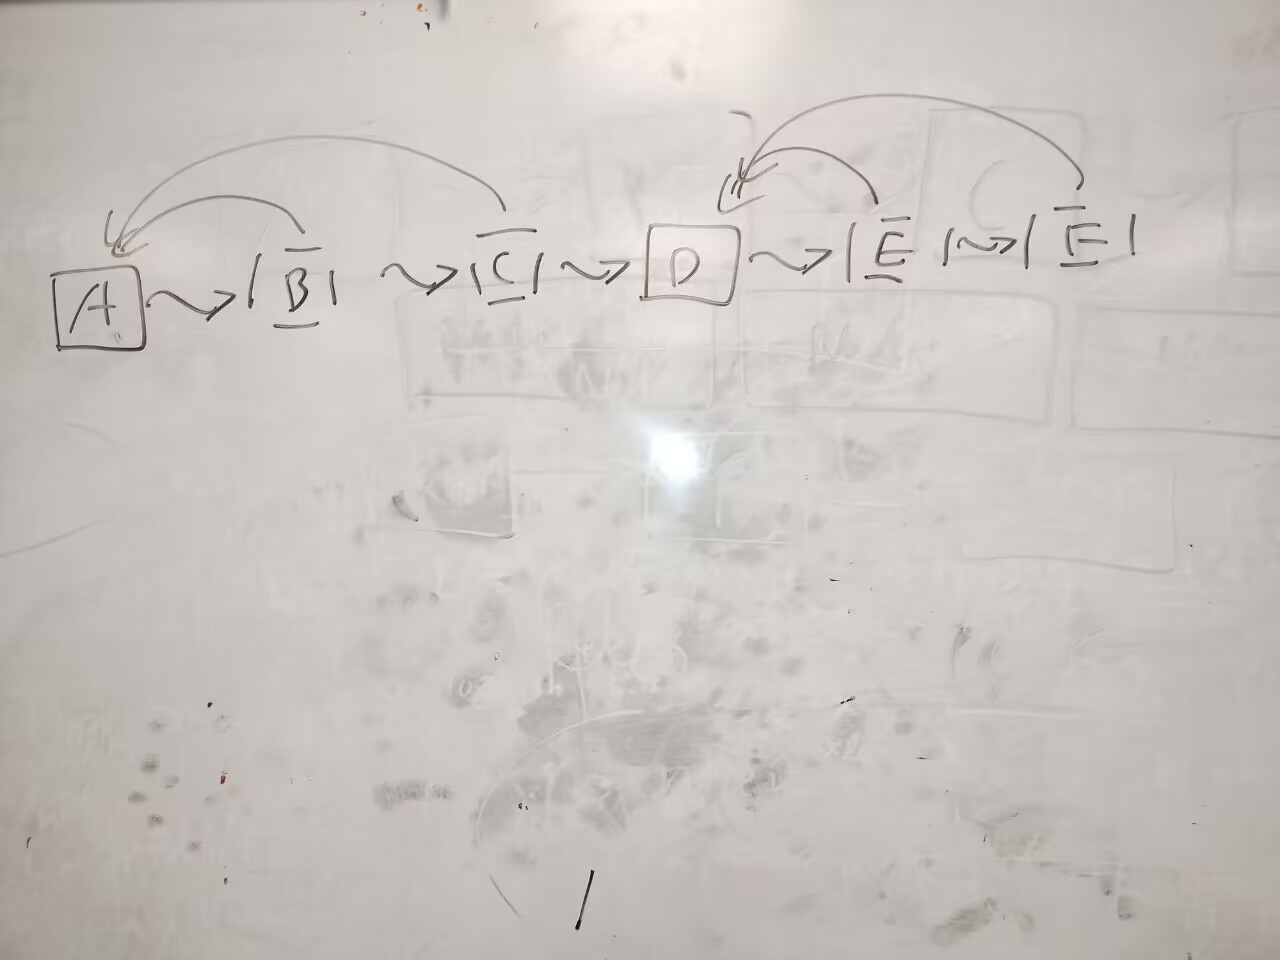
\includegraphics[width=0.5\columnwidth]{img4}
% 	\caption{lookup failure return the latest earlier node}
% \end{figure}

% \subsection{Replay Continuation}
% In order to replay for a cell at a tock t, we need to store (1) the tock t that we replay to, so we can stop once the value correspond to t is found and (2) the original state before replaying, to resume execution at that point, so we can stop once t is found, and the original state before replaying, so we can resume execution at that point. 
% This is essentially a continuation, which we called the replay continuation (RK).

% Note that it is different from the normal continuation in the following way:
% \begin{enumerate}
% 	\item continuation is a expr with a hole of type expr, while replay continuation is a state with a hole of type cell
% 	\item there are less replay continuation type then continuation: this is because only the state that lookup a cell need a replay continuation; state that does not, do not need replay, and so do not need replay continuation. An example is Eval of an function application, as it only focus on the function, pushing the arguments onto the continuation stack. 
% \end{enumerate}

% Note that, during the replaying process, more lookup might be issued, and those lookup might need more replay - replay is recursive. Just like the classical continuation at the CEK machine, the Replay Continuation need to be recursive, and form a stack as well.
% \begin{figure}
% 	\begin{tabular}{p{10em} p{2.6em} p{1em} p{0.45\textwidth}}
% 		ReplayContinuation & RK & ::= & NoReplay | Replaying Tock RH RK | \\
% 		ReplayHole & RH & ::= & RHLookup V Tock | \\
% 		& & & RHCase Env N C N C K Tock | \\
% 		& & & RHZro K Tock | RKFst K Tock | \\
% 		& & & RHApp Env E K Tock \\
% 		Replay & R & ::= & (State, RK) \\
% 	\end{tabular}
% \end{figure}

% \subsection{CEKR Machine}
% With the idea of tock, tock tree, and the replay continuation, we can now define an abstract machine, the CEKR Machine, that can uncompute and replay values.

% The CEKR Machine consist of 6 parts:
% \begin{enumerate}
% 	\item \textcolor{blue}{C}ontrol, the expression currently being evaluated.
% 	\item \textcolor{blue}{E}nvironment, a map from the free variables of the Control to their values.
% 	\item \textcolor{blue}{K}ontinuation, which is to be invoked with the value the Control evaluates to.
% 	\item \textcolor{blue}{R}eplay, the replay continuation.
% 	\item The current tock
% 	\item The tock tree
% \end{enumerate}

% In addition to the $Eval$ and $Apply$ mode in the CEK machine, there is a $Return$ mode as well. This is a ephemeral mode, indicating that we had found a cell we are replaying for, and will start playing from the top of the replay continuation at next step.

% \begin{mathpar}
%   \text{Machine} ::= (\text{State}~ | \text{Return}~ \text{Cell}), \text{rk}, \text{TockTree}
% \end{mathpar}

% \subsubsection{PostProcessing}
% The CEKR Machine execute by repeatedly computing the next node, then applying a PostProcess step. the PostProcess step have two responsibility: it insert the node onto the tock tree, and check if the node contain the cell the replay continuation is requesting. If so, it mean the current transition had found the cell we are replaying for, and our ending state should be the Return state with said cell. Otherwise, it transit to the original state.

% \begin{mathpar}
% \inferrule{ }{CheckReturn: (t, node, rk) \rightarrow State | Return cell} \and
% \inferrule{ }{CheckReturn(t, (\Nothing, st), rk) = st} \and
% \inferrule{t + 1 != t'}{CheckReturn(t, (\_, st), \NoReplay) = st} \and
% \inferrule{ }{CheckReturn(t, (\Just~ cell, st), \Replaying (t + 1) rh rk) = Return~ cell} \and
% \inferrule{t + 1 != t'}{CheckReturn(t, (\Just~ cell, st), \Replaying t' rh rk) = st} \and

% \inferrule{ }{PostProcess: (t, cell, rk, TockTree) \rightarrow Machine} \and
% \inferrule{ }{PostProcess(t, node, rk, tt) = CheckReturn(t, node, rk), rk, insert(tt, t, node)}
% \end{mathpar}

% The transition is now splitted into 3 different cases:
% \begin{enumerate}
% 	\item The happy path: in the CEKR machine, looking up from the heap is converted into querying the tock tree. The querying is successful, returning a node with a cell that match the tock we are querying, and our transition can proceed as normal, producing a node, which is a pair of cell produced and state it transit to. PostProcessing is then applied.
% 	\item The sad path: when querying fail, returning a node that does not contain a matching cell, replay is needed. To replay a cell on tock t, we push the old state alongside t onto the replay continuation, and transit to the state in the node. Note that there is no PostProcessing in this case as a node is not created.
% 	\item The return path: when the machine enter the $Return$ mode, it indicate that a query once failed, but we found the corresponding cell by replaying. By looking it up from the replay continuation, we can now re-execute the state that failed the query, as if the query result is a node containing said cell. No querying is needed in this case, as there is at most once lookup in each CEK transition, and the corresponding query had just been recomputed. Like the happy path, PostProcessing is needed to insert into the tock tree, and to recursively return.
% \end{enumerate}

% \begin{figure}
% \begin{mathpar}
% 	\inferrule{st = \Apply(cell, v, (t + 1)) \and node = (\Nothing, st)}{Return~ cell, \Replaying~ \_ (RHLookup~ v~ t) rk, tt \leadsto PostProcess(t, node, rk, tt)} \and
% 	\inferrule{st = \Eval(L, \Env[LN := X], K, (t + 1)) \and node = (\Nothing, st) \and}{Return~ (\VLeft X), \Replaying~ \_ (RHCase~ \Env~ LN~ L~ RN~ R~ K~ t), tt \leadsto PostProcess(t, node, rk, tt)} \and
% 	\inferrule{st = \Eval(R, \Env[RN := Y], K, (t + 1)) \and node = (\Nothing, st)}{Return~ (\VRight Y), \Replaying~ \_ (RHCase~ \Env~ LN~ L~ RN~ R~ K~ t), tt \leadsto PostProcess(t, node, rk, tt)} \and
% 	\inferrule{st = \Apply(K, X, (t + 1)) \and node = (\Nothing, st)}{Return~ (\VProd~ X~ Y), \Replaying~ \_ (RHZro~ K~ t), tt \leadsto PostProcess(t, node, rk, tt)} \and
% 	\inferrule{st = \Apply(K, Y, (t + 1)) \and node = (\Nothing, st)}{Return~ (\VProd~ X~ Y), \Replaying~ \_ (RHFst~ K~ t), tt \leadsto PostProcess(t, node, rk, tt)} \and
% 	\inferrule{st = \Eval(X, \Env~, (t + 1), (t + 2)) \and node = (\Just(\KApp1 \Env' N C K), st)}{Return~ (\Clos \Env'~ N~ C), \Replaying~ \_ (RHApp~ \Env~ X~ K~ t), tt \leadsto PostProcess(t, node, rk, tt)} \and	
% \end{mathpar}
% 	\caption{CEKR Transition: Returning}
% \end{figure}

% \begin{figure}
% 	\begin{mathpar}
% 		\inferrule{Query(tt, K) = (K - 1, \Just kcell) \and st = \Apply(kcell, N, t + 1) \and node = (\Nothing, st)}{\Eval(N, \Env, K, t), rk, tt \leadsto PostProcess(t, node, rk, tt)} \and
% 		\inferrule{Query(tt, K) = (X, st) \and X != K - 1}{\Eval(N, \Env, K, t), rk, tt \leadsto st, \Replaying~ K (RHLookup~ N~ t) rk, tt} \and
% 		\inferrule{st = \Eval(X, \Env, t+1, t+2) \and node = (\Just~ \KLet~A~K~C~\Env, st)}{(\Eval(\sLet~A~B~C, \Env, K, t), rk), tt \leadsto PostProcess(t, node, rk, tt)} \and
% 		\inferrule{st = \Eval(X, \Env, t+1, t+2) \and node = (\Just~ \Clos~\Env(\text{fv})\cdots N~C, st)}{(\Eval(\sLam~N~C, \Env, K, t), rk), tt \leadsto PostProcess(t, node, rk, tt)} \and
% 		\inferrule{st = \Eval(X, \Env, t+1, t+2) \and node = (\Just~ \KApp_0~\Env~X~K, st)}{(\Eval(\sApp~F~X, \Env, K, t), rk), tt \leadsto PostProcess(t, node, rk, tt)} \and
% 		\inferrule{st = \Eval(X, \Env, t+1, t+2) \and node = (\Just~ \KProd_0~K~R, st)}{(\Eval(\sProd~L~R, \Env, K, t), rk), tt \leadsto PostProcess(t, node, rk, tt)} \and
% 		\inferrule{st = \Eval(X, \Env, t+1, t+2) \and node = (\Just~ \KZro~K, st)}{(\Eval(\sZro~X, \Env, K, t), rk), tt \leadsto PostProcess(t, node, rk, tt)} \and
% 		\inferrule{st = \Eval(X, \Env, t+1, t+2) \and node = (\Just~ \KFst~K, st)}{(\Eval(\sFst~X, \Env, K, t), rk), tt \leadsto PostProcess(t, node, rk, tt)} \and
% 		\inferrule{st = \Eval(X, \Env, t+1, t+2) \and node = (\Just~ \KLeft~K, st)}{(\Eval(\sLeft~X, \Env, K, t), rk), tt \leadsto PostProcess(t, node, rk, tt)} \and
% 		\inferrule{st = \Eval(X, \Env, t+1, t+2) \and node = (\Just~ \KRight~K, st)}{(\Eval(\sRight~X, \Env, K, t), rk), tt \leadsto PostProcess(t, node, rk, tt)} \and
% 		\inferrule{st = \Eval(X, \Env, t+1, t+2) \and node = (\Just~ \KCase~\mathit{LN}~L~\mathit{RN}~R~\Env, st)}{(Eval(\sCase~X~\mathit{LN}~L~\mathit{RN}~R, \Env, K, t), rk), tt \leadsto PostProcess(t, node, rk, tt)} \and
% 	\end{mathpar}
% 	\caption{CEKR Transition: Eval}
% \end{figure}
% \begin{figure}
% 	\begin{mathpar}
% 		\inferrule{Query(tt, K) = (X, (\_, st)) \and X != K - 1}{\Apply(\KLookup K, V, t, rk), tt \leadsto st, \Replaying~ K~ (RHLookup V t) rk, tt} \and
% 		\inferrule{Query(tt, K) = (K - 1, (\Just cell, \_)) \and st = \Apply(cell, V, t+1) \and node = (\Nothing, st)}{\Apply(\KLookup K, V, t), rk, tt \leadsto PostProcess(t, node, rk, tt)} \and
% 		\inferrule{st = \Eval(C, Env[A := V], K', t+1) \and node = (Nothing, st) }{\Apply(\KLet~ A~ \Env~ C~ K', V, t), rk, tt \leadsto PostProcess(t, node, rk, tt)} \and
% 		\inferrule{Query(tt, V) = (X', (\_, st)) \and X' != V - 1}{(Apply(\Just~ KApp0 Env X K, V, t), rk), tt \leadsto st, \Replaying V (RHApp Env X K t) rk, tt} \and
% 		\inferrule{Query(tt, V) = (V - 1, (\Clos Env' N C), \_) \and st = \Eval(X, Env, t+1, t+2) \and node = (\Just KApp1 \Env' N C K', st)}{\Apply(\KApp0~ \Env~ X~ K', V, t), rk, tt \leadsto PostProcess(t, node, rk, tt)} \and
% 		\inferrule{st = \Eval(C, Env[N := V], K', t+1) \and node = (Nothing, st)}{\Apply(\KApp1 Env N C K', V, t), rk, tt \leadsto PostProcess(t, node, rk, tt)} \and
% 		\inferrule{st = \Eval(R, Env, t+1, t+2) \and node = (\Just KProd1 V Env K, st)}{\Apply(KProd0 Env R K, V, t), rk, tt \leadsto PostProcess(t, node, rk, tt)} \and
% 		\inferrule{st = \Apply(K, t+1, t+2) \and node = (\Just \VProd L V, st)}{Apply(KProd1 L K, V, t), rk, TT \leadsto PostProcess(t, node, rk, tt)} \and
% 		\inferrule{Query(tt, V) = (X, (\_, st)) \and X != V - 1}{Apply(KZro K, V, t), rk, tt \leadsto st, \Replaying~ V~ (RHZro K t) rk, tt} \and
% 		\inferrule{Query(tt, V) = (V - 1, (VProd X Y, \_)) \and st = \Apply(K, X, t+1) \and node = (\Nothing, st)}{Apply(KZro K, V, t), rk, tt \leadsto PostProcess(t, node, rk, tt)} \and
% 		\inferrule{Query(tt, V) = (X, (\_, st)) \and X != V - 1}{\Apply(KFst K, V, t), rk, tt \leadsto st, \Replaying~ V~ (RHFst K t) rk, tt} \and
% 		\inferrule{Query(tt, V) = (V - 1, (VProd X Y, \_)) \and st = \Apply(K, Y, t+1) \and node = (Nothing, st)}{\Apply(KFst K, V, t), rk, tt \leadsto PostProcess(t, node, rk, tt)} \and
% 	\end{mathpar}
% 	\caption{CEKR Transition: Apply}
% \end{figure}
% \begin{figure}
% 	\begin{mathpar}
% 		\inferrule{st = \Apply(K, t+1, t+2) \and node = (\Just~ VLeft V, st)}{\Apply(KLeft K, V, t), rk, tt \leadsto PostProcess(t, node, rk, tt)} \and
% 		\inferrule{st = \Apply(K, t+1, t+2) \and node = (\Just~ VRight V, st)}{\Apply(KRight K, V, t), rk, tt \leadsto PostProcess(t, node, rk, tt)} \and
% 		\inferrule{Query(tt, V) = (X, (\_, st)) \and X != V - 1}{\Apply(KCase Env LN L RN R K, V, t), rk, tt \leadsto st, \Replaying V (RHCase Env LN L RN R K t) rk), tt} \and
% 		\inferrule{Query(tt, V) = (V - 1, (\Just~ VLeft X, \_)) \and st = \Eval(L, \Env[LN := X], K', t+1) \and node = (Nothing, st)}{Apply(KCase Env LN L RN R K, V, t), rk, tt \leadsto PostProcess(t, node, rk, tt)} \and
% 		\inferrule{Query(tt, V) = (V - 1, (\Just~ VRight Y, \_)) \and st = \Eval(R, \Env[RN := Y], K', t+1) \and node = (Nothing, st)}{Apply(KCase Env LN L RN R K, V, t), rk, tt \leadsto PostProcess(t, node, rk, tt)} \and
% 	\end{mathpar}
% 	\caption{CEKR Transition: Apply}
% \end{figure}

\section{Uncomputing and Recomputing}
\subsection{Tock}
The key insight of Zombie is to introduce an abstraction layer between the executing program and the heap. This abstraction layer will allow the heap to transparently discard and recompute the program's intermediate values. To do so, we use the CEK machine to refer to each intermediate value by the index of the computation step that created it. Since each CEK step allocates at most one cell, this correspondence is injective. In other words, instead of storing pointers that refer to memory locations, we will store pointers, which we call ``tocks'', that refer to points in time---that is, CEK step indices.

In our runtime, these ``tocks'' are implemented as 64-bit integers, though in our model we will treat them as logically unbounded integers. There is a global ``current tock'' counter, which starts at 0 and is increased by 1 at every transition step in the abstract machine and every allocation. The cell allocated at step $i$ is then referred to by the tock $i$, and that tock can then be used as a pointer, stored in data structures, looked up by later computations steps, and the like.

Note that, due to the determinism and linearity of the CEK machine, tocks are strictly ordered and the value computed at some tock $i$ can only depend on values computed at earlier tocks. Moreover, we can recreate the value at tock $i$ by merely rerunning the CEK machine from some earlier state to that point. Because the CEK machine is deterministic, this re-execution will produce the same exact value as the original. Because our pointers refer to abstract values, not to specific memory locations, the heap can thus re-compute a value as necessary instead of storing it in memory.

In other words, the way Zombie works is that the heap will store only some of the intermediate values. The ones that aren't stored will instead be recomputed as needed, and the heap will store earlier CEK states to facilitate that. As the program runs, intermediate values can be discarded from the heap to reduce its memory usage.

Because a value can be recomputed from \emph{any} earlier CEK state, it will also turn out to be possible to store relatively few states. Therefore, overall memory usage---for the stored intermediate values and the stored states---can be kept low. In Zombie, we can store asymptotically fewer states than intermediate values, allowing us to asymptotically reduce memory usage.

\subsection{Tock Tree}
In Zombie, the heap is implemented by a runtime data structure called the tock tree. The tock tree maps tocks to the cells allocated by that step; in other words, the tock tree implements the mapping between tocks and their actual memory locations. Because values can be evicted to save memory, however, not all tocks have a mapping in the tock tree. Instead, every tock that \emph{is} present in the tock tree will also store its state. To recompute an evicted value at some tock $i$, the tock tree will find the largest state at tock $j < i$ and replay from that tock to tock $i$.

Each node in the Tock Tree stores both a memory cell and a state. Specifically, consider the execution of the CEK machine from step $t$. In step $t + 1$ it allocates a cell; it then performs a computation in step $t + 2$. So the node at tock $t$ contains both the cell allocated at step $t + 1$ as well as the state \emph{afterward}, at step $t + 2$. A transition might not allocate any new cells, in such a case the Node only stores a state and no memory cell. To be more specific, if the node represents the execution of the CEK machine at step $t$, it will only contain the CEK state at step $t + 1$. Also note that a state, in this context, does not include every info needed for execution: in particular it does not include the tock tree, alongside any data that guide recomputation. More specifically a state denotes either a $\Eval~C~\Env~K~Tock$ or a $\Apply~K~V~Tock$.

One thing worth noticing is that continuations are also reified. This means we treat them as like values, lifting pointers into tock, and storing continuations onto the tock tree. This allows us to also uncompute continuation as well, by evicting the node on the tock tree holding said continuation. This is crucial as traversing a deep data structure non-tail-recursively produces a continuation chain of equal depth. In contrast to a ordinary runtime, in which this is a slight but inevitable unfortunate, in our case, the continuation storage can become the bottleneck of the system.

In order to make this operation efficient, the tock tree is organized as a binary search tree. In a binary search tree, arbitrary keys (tocks) can be looked up in $O(\log(n))$ time, where $n$ is the size of the tock tree, and when a key is not found, the largest key smaller than it can be easily found. Then the heap can replay execution from that point to compute the desired tock.

\begin{figure}
    \begin{tabular}{p{5em} p{3em} p{10em} p{0.45\textwidth}}
        Value & = & \st{P<VCell>} & Tock \\
        Continuation & = & \st{P<KCell>} & Tock \\
        State & ::= & \st{$\Eval~C~\Env~K \mid \Apply~K~V $} & $\Eval~C~\Env~K~Tock \mid \Apply~K~V~Tock $ \\
        Node & = & & (Maybe(KCell | VCell), State) \\
        Query & $:$ & (TockTree, Tock) & -> (Tock, Node) \\
        Insert & $:$ & (TockTree, Tock, Node) & -> TockTree \\
    \end{tabular}
    \caption{Tock Tree API. Note that we deliberately avoid dictating what node gets uncomputed, to decouple uncomputation/recomputation with selecting what to uncompute. Instead, a node might be dropped during insertion into TockTree. One might e.g. set a limit on the amount of nodes in the Tock Tree. }
\end{figure}
\begin{figure}
    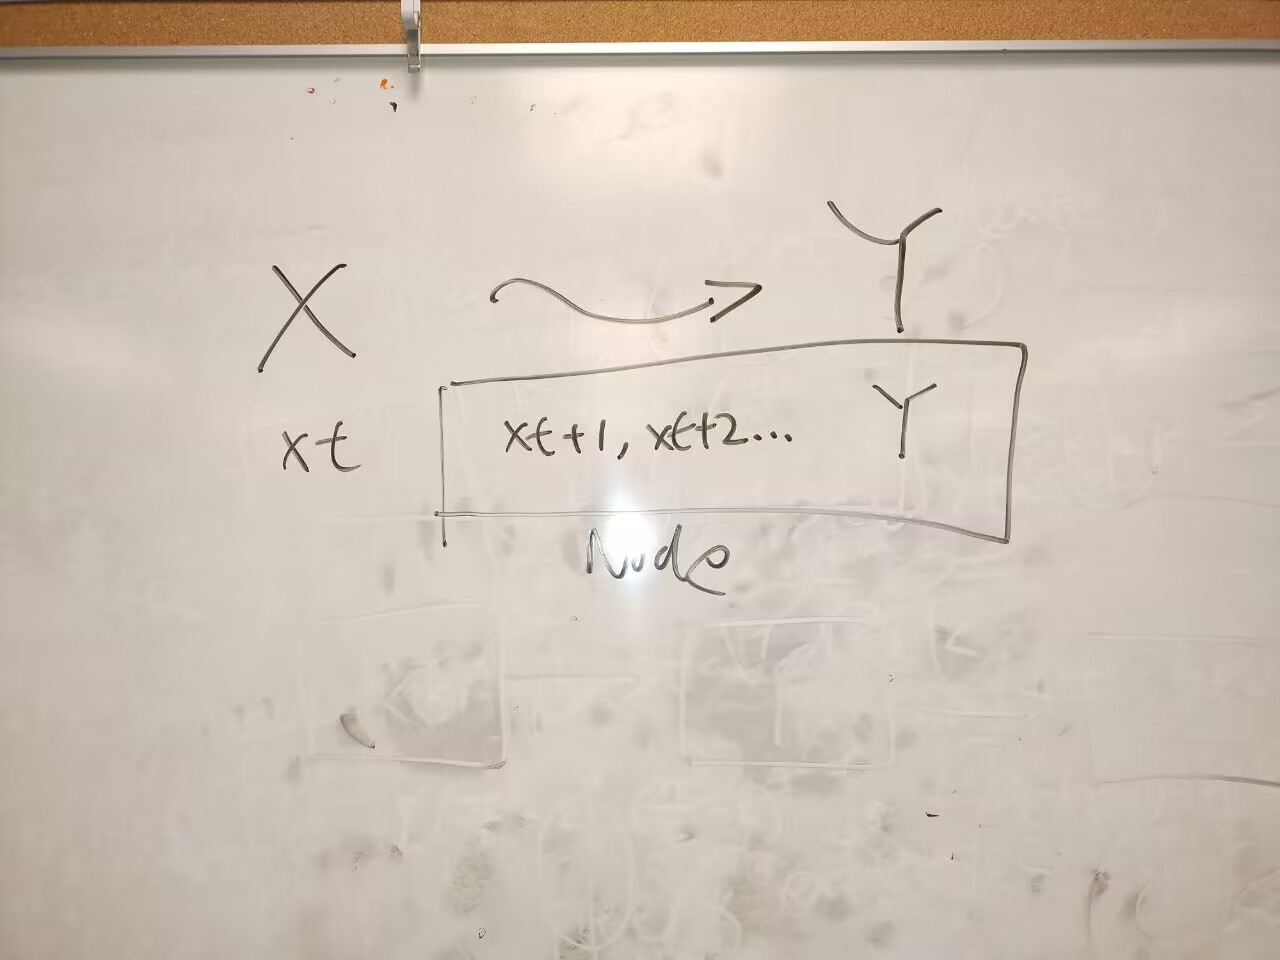
\includegraphics[width=0.5\columnwidth]{img2}
    \caption{a node in the tock tree}
\end{figure}
\begin{figure}
    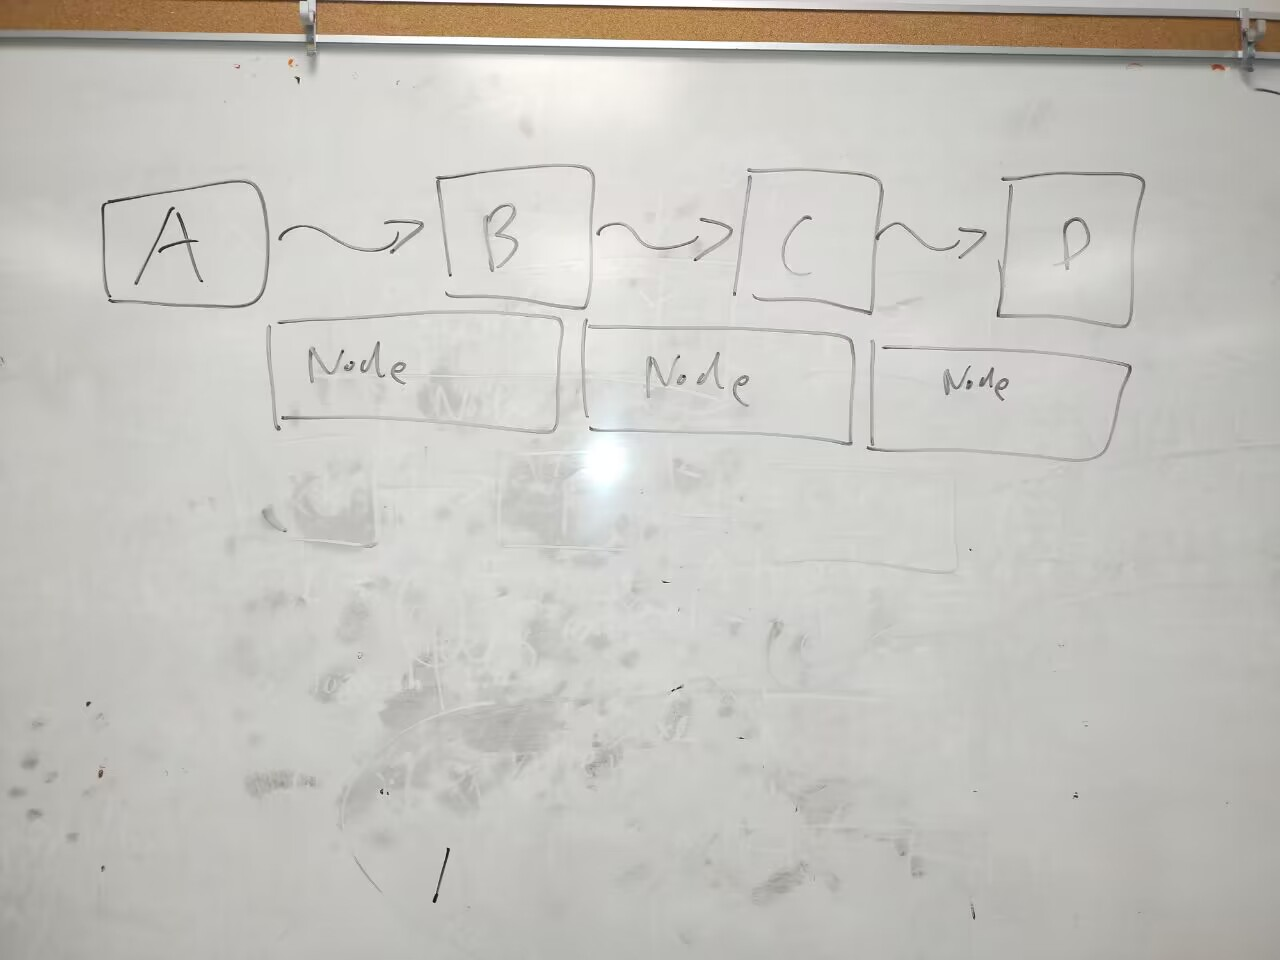
\includegraphics[width=0.5\columnwidth]{img3}
    \caption{the tock tree with multiple nodes}
\end{figure}

\begin{figure}
    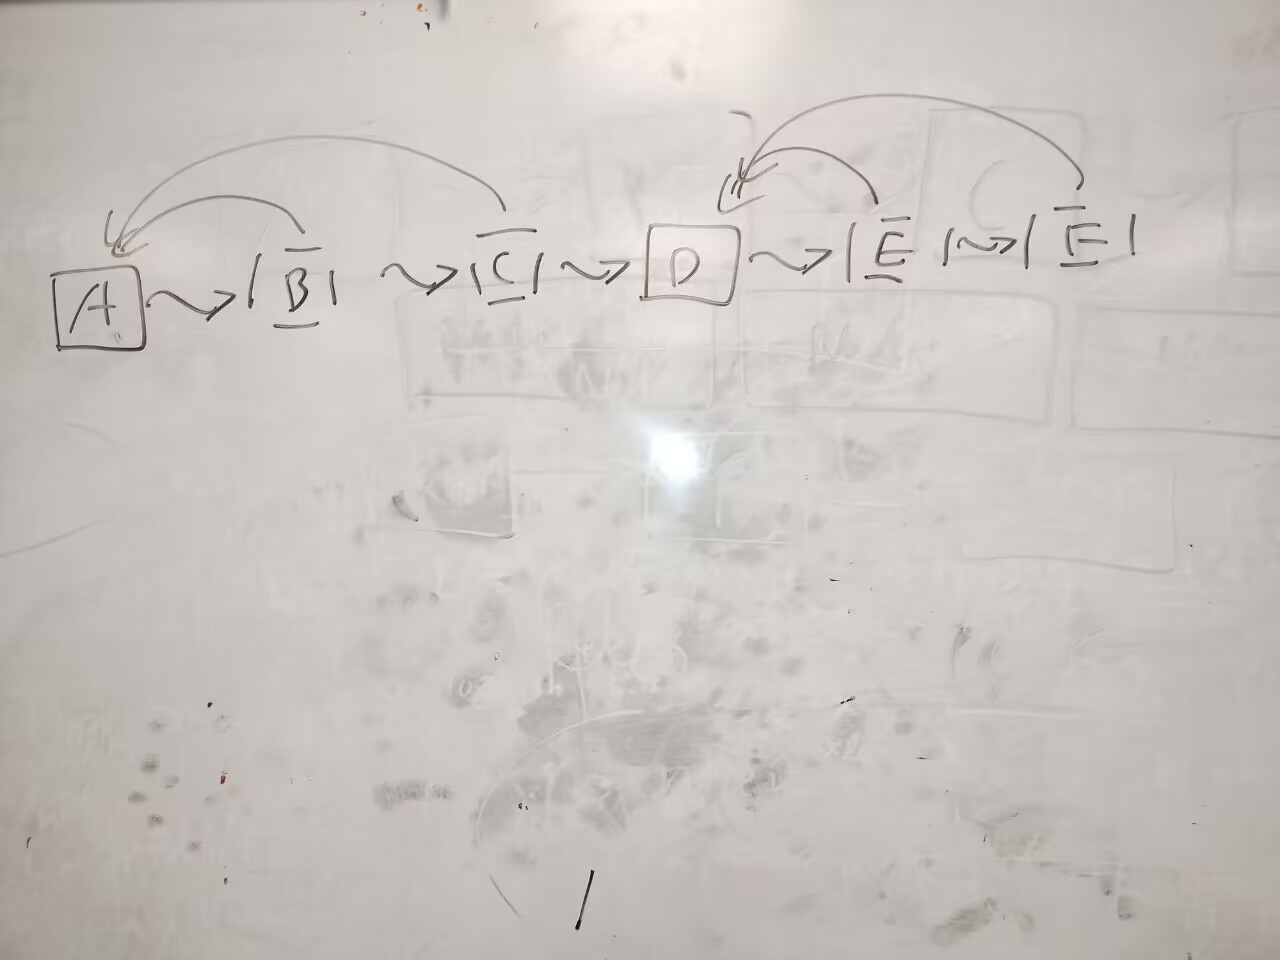
\includegraphics[width=0.5\columnwidth]{img4}
    \caption{lookup failure return the latest earlier node}
\end{figure}

\subsection{Replay Continuation}
In order to replay for a cell at a tock t, we need to store (1) the tock t that we replay to, so we can stop once the value corresponding to t is found and (2) the original state before replaying, resume execution at that point, so we can stop once t is found, and the original state before replaying, so we can resume execution at that point. 
This is essentially a continuation, which we call the replay continuation (RK).

Note that it is different from the normal continuation in the following way:
\begin{enumerate}
    \item continuation is an expr with a hole of type expr, while replay continuation is a state with a hole of type cell
    \item there are fewer replay continuation types than continuation: this is because only the state that lookup a cell needs a replay continuation; a state that does not, does not need a replay, and so does not need replay continuation. An example is Eval of a function application, as it only focuses on the function, pushing the arguments onto the continuation stack. 
\end{enumerate}

Note that, during the replaying process, more lookups might be issued, and those lookups might need more replay - replay is recursive. Just like the classical continuation at the CEK machine, the Replay Continuation needs to be recursive and form a stack as well.
\begin{figure}
    \begin{tabular}{p{10em} p{2.6em} p{1em} p{0.45\textwidth}}
        ReplayContinuation & RK & ::= & NoReplay | Replaying Tock RH RK | \\
        ReplayHole & RH & ::= & RHLookup V Tock | \\
        & & & RHCase Env N C N C K Tock | \\
        & & & RHZro K Tock | RKFst K Tock | \\
        & & & RHApp Env E K Tock \\
        Replay & R & ::= & (State, RK) \\
    \end{tabular}
\end{figure}

\subsection{CEKR Machine}
With the idea of tock, tock tree, and the replay continuation, we can now define an abstract machine, the CEKR Machine, that can uncompute and replay values.

The CEKR Machine consists of 6 parts:
\begin{enumerate}
    \item \textcolor{blue}{C}ontrol, the expression currently being evaluated.
    \item \textcolor{blue}{E}nvironment, a map from the free variables of the Control to their values.
    \item \textcolor{blue}{K}ontinuation, which is to be invoked with the value the Control evaluates to.
    \item \textcolor{blue}{R}eplay, the replay continuation.
    \item The current tock
    \item The tock tree
\end{enumerate}

In addition to the $Eval$ and $Apply$ modes in the CEK machine, there is a $Return$ mode as well. This is an ephemeral mode, indicating that we have found a cell we are replaying for and will start playing from the top of the replay continuation at the next step.

\begin{mathpar}
  \text{Machine} ::= (\text{State}~ | \text{Return}~ \text{Cell}), \text{rk}, \text{TockTree}
\end{mathpar}

\subsubsection{PostProcessing}
The CEKR Machine executes by repeatedly computing the next node, and then applying a PostProcess step. the PostProcess step has two responsibilities: it inserts the node onto the tock tree, and checks if the node contains the cell the replay continuation is requesting. If so, it means the current transition has found the cell we are replaying for, and our ending state should be the Return state with said cell. Otherwise, it transits to the original state.

\begin{mathpar}
\inferrule{ }{CheckReturn: (t, node, rk) \rightarrow State | Return cell} \and
\inferrule{ }{CheckReturn(t, (\Nothing, st), rk) = st} \and
\inferrule{t + 1 != t'}{CheckReturn(t, (\_, st), \NoReplay) = st} \and
\inferrule{ }{CheckReturn(t, (\Just~ cell, st), \Replaying (t + 1) rh rk) = Return~ cell} \and
\inferrule{t + 1 != t'}{CheckReturn(t, (\Just~ cell, st), \Replaying t' rh rk) = st} \and

\inferrule{ }{PostProcess: (t, cell, rk, TockTree) \rightarrow Machine} \and
\inferrule{ }{PostProcess(t, node, rk, tt) = CheckReturn(t, node, rk), rk, insert(tt, t, node)}
\end{mathpar}

The transition is now split into 3 different cases:
\begin{enumerate}
    \item The happy path: in the CEKR machine, looking up from the heap is converted into querying the tock tree. The querying is successful, returning a node with a cell that matches the tock we are querying, and our transition can proceed as normal, producing a node, which is a pair of the cell produced and the state it transits to. PostProcessing is then applied.
    \item The sad path: when querying fails, returning a node that does not contain a matching cell, replay is needed. To replay a cell on tock t, we push the old state alongside t onto the replay continuation, and transit to the state in the node. Note that there is no PostProcessing in this case as a node is not created.
    \item The return path: when the machine enters the $Return$ mode, it indicates that a query once failed, but we found the corresponding cell by replaying. By looking it up from the replay continuation, we can now re-execute the state that failed the query, as if the query result is a node containing said cell. No querying is needed in this case, as there is at most one lookup in each CEK transition, and the corresponding query had just been recomputed. Like the happy path, PostProcessing is needed to insert into the tock tree and to recursively return.
\end{enumerate}

\begin{figure}
\begin{mathpar}
    \inferrule{st = \Apply(cell, v, (t + 1)) \and node = (\Nothing, st)}{Return~ cell, \Replaying~ \_ (RHLookup~ v~ t) rk, tt \leadsto PostProcess(t, node, rk, tt)} \and
    \inferrule{st = \Eval(L, \Env[LN := X], K, (t + 1)) \and node = (\Nothing, st) \and}{Return~ (\VLeft X), \Replaying~ \_ (RHCase~ \Env~ LN~ L~ RN~ R~ K~ t), tt \leadsto PostProcess(t, node, rk, tt)} \and
    \inferrule{st = \Eval(R, \Env[RN := Y], K, (t + 1)) \and node = (\Nothing, st)}{Return~ (\VRight Y), \Replaying~ \_ (RHCase~ \Env~ LN~ L~ RN~ R~ K~ t), tt \leadsto PostProcess(t, node, rk, tt)} \and
    \inferrule{st = \Apply(K, X, (t + 1)) \and node = (\Nothing, st)}{Return~ (\VProd~ X~ Y), \Replaying~ \_ (RHZro~ K~ t), tt \leadsto PostProcess(t, node, rk, tt)} \and
    \inferrule{st = \Apply(K, Y, (t + 1)) \and node = (\Nothing, st)}{Return~ (\VProd~ X~ Y), \Replaying~ \_ (RHFst~ K~ t), tt \leadsto PostProcess(t, node, rk, tt)} \and
    \inferrule{st = \Eval(X, \Env~, (t + 1), (t + 2)) \and node = (\Just(\KApp1 \Env' N C K), st)}{Return~ (\Clos \Env'~ N~ C), \Replaying~ \_ (RHApp~ \Env~ X~ K~ t), tt \leadsto PostProcess(t, node, rk, tt)} \and   
\end{mathpar}
    \caption{CEKR Transition: Returning}
\end{figure}

\begin{figure}
    \begin{mathpar}
        \inferrule{Query(tt, K) = (K - 1, \Just kcell) \and st = \Apply(kcell, N, t + 1) \and node = (\Nothing, st)}{\Eval(N, \Env, K, t), rk, tt \leadsto PostProcess(t, node, rk, tt)} \and
        \inferrule{Query(tt, K) = (X, st) \and X != K - 1}{\Eval(N, \Env, K, t), rk, tt \leadsto st, \Replaying~ K (RHLookup~ N~ t) rk, tt} \and
        \inferrule{st = \Eval(X, \Env, t+1, t+2) \and node = (\Just~ \KLet~A~K~C~\Env, st)}{(\Eval(\sLet~A~B~C, \Env, K, t), rk), tt \leadsto PostProcess(t, node, rk, tt)} \and
        \inferrule{st = \Eval(X, \Env, t+1, t+2) \and node = (\Just~ \Clos~\Env(\text{fv})\cdots N~C, st)}{(\Eval(\sLam~N~C, \Env, K, t), rk), tt \leadsto PostProcess(t, node, rk, tt)} \and
        \inferrule{st = \Eval(X, \Env, t+1, t+2) \and node = (\Just~ \KApp_0~\Env~X~K, st)}{(\Eval(\sApp~F~X, \Env, K, t), rk), tt \leadsto PostProcess(t, node, rk, tt)} \and
        \inferrule{st = \Eval(X, \Env, t+1, t+2) \and node = (\Just~ \KProd_0~K~R, st)}{(\Eval(\sProd~L~R, \Env, K, t), rk), tt \leadsto PostProcess(t, node, rk, tt)} \and
        \inferrule{st = \Eval(X, \Env, t+1, t+2) \and node = (\Just~ \KZro~K, st)}{(\Eval(\sZro~X, \Env, K, t), rk), tt \leadsto PostProcess(t, node, rk, tt)} \and
        \inferrule{st = \Eval(X, \Env, t+1, t+2) \and node = (\Just~ \KFst~K, st)}{(\Eval(\sFst~X, \Env, K, t), rk), tt \leadsto PostProcess(t, node, rk, tt)} \and
        \inferrule{st = \Eval(X, \Env, t+1, t+2) \and node = (\Just~ \KLeft~K, st)}{(\Eval(\sLeft~X, \Env, K, t), rk), tt \leadsto PostProcess(t, node, rk, tt)} \and
        \inferrule{st = \Eval(X, \Env, t+1, t+2) \and node = (\Just~ \KRight~K, st)}{(\Eval(\sRight~X, \Env, K, t), rk), tt \leadsto PostProcess(t, node, rk, tt)} \and
        \inferrule{st = \Eval(X, \Env, t+1, t+2) \and node = (\Just~ \KCase~\mathit{LN}~L~\mathit{RN}~R~\Env, st)}{(Eval(\sCase~X~\mathit{LN}~L~\mathit{RN}~R, \Env, K, t), rk), tt \leadsto PostProcess(t, node, rk, tt)} \and
    \end{mathpar}
    \caption{CEKR Transition: Eval}
\end{figure}
\begin{figure}
    \begin{mathpar}
        \inferrule{Query(tt, K) = (X, (\_, st)) \and X != K - 1}{\Apply(\KLookup K, V, t, rk), tt \leadsto st, \Replaying~ K~ (RHLookup V t) rk, tt} \and
        \inferrule{Query(tt, K) = (K - 1, (\Just cell, \_)) \and st = \Apply(cell, V, t+1) \and node = (\Nothing, st)}{\Apply(\KLookup K, V, t), rk, tt \leadsto PostProcess(t, node, rk, tt)} \and
        \inferrule{st = \Eval(C, Env[A := V], K', t+1) \and node = (Nothing, st) }{\Apply(\KLet~ A~ \Env~ C~ K', V, t), rk, tt \leadsto PostProcess(t, node, rk, tt)} \and
        \inferrule{Query(tt, V) = (X', (\_, st)) \and X' != V - 1}{(Apply(\Just~ KApp0 Env X K, V, t), rk), tt \leadsto st, \Replaying V (RHApp Env X K t) rk, tt} \and
        \inferrule{Query(tt, V) = (V - 1, (\Clos Env' N C), \_) \and st = \Eval(X, Env, t+1, t+2) \and node = (\Just KApp1 \Env' N C K', st)}{\Apply(\KApp0~ \Env~ X~ K', V, t), rk, tt \leadsto PostProcess(t, node, rk, tt)} \and
        \inferrule{st = \Eval(C, Env[N := V], K', t+1) \and node = (Nothing, st)}{\Apply(\KApp1 Env N C K', V, t), rk, tt \leadsto PostProcess(t, node, rk, tt)} \and
        \inferrule{st = \Eval(R, Env, t+1, t+2) \and node = (\Just KProd1 V Env K, st)}{\Apply(KProd0 Env R K, V, t), rk, tt \leadsto PostProcess(t, node, rk, tt)} \and
        \inferrule{st = \Apply(K, t+1, t+2) \and node = (\Just \VProd L V, st)}{Apply(KProd1 L K, V, t), rk, TT \leadsto PostProcess(t, node, rk, tt)} \and
        \inferrule{Query(tt, V) = (X, (\_, st)) \and X != V - 1}{Apply(KZro K, V, t), rk, tt \leadsto st, \Replaying~ V~ (RHZro K t) rk, tt} \and
        \inferrule{Query(tt, V) = (V - 1, (VProd X Y, \_)) \and st = \Apply(K, X, t+1) \and node = (\Nothing, st)}{Apply(KZro K, V, t), rk, tt \leadsto PostProcess(t, node, rk, tt)} \and
        \inferrule{Query(tt, V) = (X, (\_, st)) \and X != V - 1}{\Apply(KFst K, V, t), rk, tt \leadsto st, \Replaying~ V~ (RHFst K t) rk, tt} \and
        \inferrule{Query(tt, V) = (V - 1, (VProd X Y, \_)) \and st = \Apply(K, Y, t+1) \and node = (Nothing, st)}{\Apply(KFst K, V, t), rk, tt \leadsto PostProcess(t, node, rk, tt)} \and
    \end{mathpar}
    \caption{CEKR Transition: Apply}
\end{figure}
\begin{figure}
    \begin{mathpar}
        \inferrule{st = \Apply(K, t+1, t+2) \and node = (\Just~ VLeft V, st)}{\Apply(KLeft K, V, t), rk, tt \leadsto PostProcess(t, node, rk, tt)} \and
        \inferrule{st = \Apply(K, t+1, t+2) \and node = (\Just~ VRight V, st)}{\Apply(KRight K, V, t), rk, tt \leadsto PostProcess(t, node, rk, tt)} \and
        \inferrule{Query(tt, V) = (X, (\_, st)) \and X != V - 1}{\Apply(KCase Env LN L RN R K, V, t), rk, tt \leadsto st, \Replaying V (RHCase Env LN L RN R K t) rk), tt} \and
        \inferrule{Query(tt, V) = (V - 1, (\Just~ VLeft X, \_)) \and st = \Eval(L, \Env[LN := X], K', t+1) \and node = (Nothing, st)}{Apply(KCase Env LN L RN R K, V, t), rk, tt \leadsto PostProcess(t, node, rk, tt)} \and
        \inferrule{Query(tt, V) = (V - 1, (\Just~ VRight Y, \_)) \and st = \Eval(R, \Env[RN := Y], K', t+1) \and node = (Nothing, st)}{Apply(KCase Env LN L RN R K, V, t), rk, tt \leadsto PostProcess(t, node, rk, tt)} \and
    \end{mathpar}
    \caption{CEKR Transition: Apply}
\end{figure}

